% SDRTerm — ADS-B reception range: how far can you actually hear?
%
% Build with:  pdflatex range.tex  (twice, so refs resolve)

\documentclass[11pt,a4paper]{article}

\usepackage[margin=2cm]{geometry}
\usepackage{amsmath,amssymb}
\usepackage{tikz}
\usepackage{pgfplots}
\pgfplotsset{compat=1.18}
\usetikzlibrary{arrows.meta, positioning, calc, decorations.pathreplacing}
\usepackage{siunitx}
\usepackage{hyperref}
\usepackage{parskip}
\usepackage{booktabs}

\hypersetup{colorlinks=true, linkcolor=blue!70!black, urlcolor=blue!60!black}

\title{ADS-B Reception Range\\
       \large A geometric first pass, plus every side effect worth naming}
\author{SDRTerm project}
\date{\today}

\begin{document}
\maketitle
\tableofcontents
\vspace{1em}

%═══════════════════════════════════════════════════════════════════
\section{Introduction}
%═══════════════════════════════════════════════════════════════════

You are at $\phi = \ang{49.740693}$\,N, $\lambda = \ang{6.660242}$\,E ---
the Trier area of western Germany, sitting in the Moselle valley at
about \SI{150}{m} above mean sea level.  1090\,MHz ADS-B squitters
from commercial aircraft carry usable data whenever a straight line
can be drawn between the aircraft's antenna and yours.  How far away
does that limit sit?

The rest of this note takes the question apart, layer by layer:
first pure geometry (\S\ref{sec:geom}), then the standard atmospheric
correction (\S\ref{sec:refraction}), then the link-budget check that
confirms the geometric limit is what actually binds you (\S\ref{sec:link}),
and finally a tour of the smaller effects --- diffraction, ducting,
Doppler, relativity, terrain --- that either matter for edge cases
or that people bring up but are actually negligible at 1090\,MHz.

%═══════════════════════════════════════════════════════════════════
\section{Geometry only: the radio horizon}\label{sec:geom}
%═══════════════════════════════════════════════════════════════════

Pretend the earth is a smooth sphere of radius $R = \SI{6371}{km}$ and
the atmosphere doesn't bend anything.  The reception limit is then the
classical \emph{radio horizon}: the range at which the aircraft's antenna
first pokes above your local horizon plane.

\begin{center}
\begin{tikzpicture}[scale=1.0]
  % Earth as a large circle arc
  \begin{scope}
    \clip (-6,-0.05) rectangle (6,4);
    \draw[thick, blue!30!black, fill=blue!5] (0,-15) circle (15);
  \end{scope}
  % Receiver on the surface
  \filldraw[green!50!black] (-3.2,{sqrt(225 - 3.2*3.2) - 15}) circle (0.06)
    node[above=1pt, font=\scriptsize] {you $(h_r)$};
  % Aircraft above the surface
  \filldraw[red] (3.2, 1.2) circle (0.08)
    node[above=1pt, font=\scriptsize] {aircraft $(h_t)$};
  % Line-of-sight tangent
  \draw[dashed, red!70!black, thick]
    (-3.2,{sqrt(225 - 3.2*3.2) - 15}) -- (3.2, 1.2);
  % Horizon labels + tangent point
  \filldraw[gray] (0,0) circle (0.04) node[below=1pt, font=\tiny] {horizon};
  \draw[decorate, decoration={brace, amplitude=4pt},
        gray] (-3.2, -0.15) -- (0, -0.15)
    node[midway, below=6pt, font=\tiny]{$\sqrt{2 R h_r}$};
  \draw[decorate, decoration={brace, amplitude=4pt},
        gray] (0, -0.15) -- (3.2, -0.15)
    node[midway, below=6pt, font=\tiny]{$\sqrt{2 R h_t}$};
\end{tikzpicture}
\end{center}

For an object at height $h$ above the sphere, the distance from the object
to the tangent point on the surface is
\begin{equation}
d \;=\; \sqrt{h\,(2R + h)}
   \;\approx\; \sqrt{2 R h} \qquad (h \ll R).
\end{equation}
A receiver at $h_r$ and a transmitter at $h_t$ can just see each other
when the sum of the two horizon distances equals their separation:
\begin{equation}\label{eq:horizon}
\boxed{\;d_{\max} \;=\; \sqrt{2 R h_r} \;+\; \sqrt{2 R h_t}\;}
\end{equation}

\subsection{Numbers for your setup}

Take $R = \SI{6371}{km}$.  Each column of the table below is one term of
\eqref{eq:horizon} evaluated separately.

\begin{center}
\begin{tabular}{l r r}
\toprule
Scenario                                      & Height above MSL & Horizon term  \\
\midrule
\multicolumn{3}{l}{\emph{Receiver}} \\
Attic antenna on a house,   \SI{5}{m} pole    & \SI{5}{m}        & \SI{8.0}{km}   \\
Rural Trier area (typical)                    & \SI{150}{m}      & \SI{43.7}{km}  \\
Nearby hilltop (Petrisberg, Grüneberg)        & \SI{400}{m}      & \SI{71.4}{km}  \\
\midrule
\multicolumn{3}{l}{\emph{Aircraft}} \\
Regional turboprop,     \SI{20000}{ft}         & \SI{6096}{m}     & \SI{278}{km}   \\
Airliner cruise low,    \SI{30000}{ft}         & \SI{9144}{m}     & \SI{341}{km}   \\
Airliner cruise mid,    \SI{35000}{ft}         & \SI{10668}{m}    & \SI{368}{km}   \\
Airliner cruise high,   \SI{40000}{ft}         & \SI{12192}{m}    & \SI{394}{km}   \\
Long-haul step-climb,   \SI{45000}{ft}         & \SI{13716}{m}    & \SI{418}{km}   \\
\bottomrule
\end{tabular}
\end{center}

Combining a receiver at \SI{150}{m} with a jet at \SI{40000}{ft}:
\[
d_{\max} \;=\; \SI{43.7}{km} \,+\, \SI{394}{km}
         \;\approx\; \boxed{\SI{438}{km}}
\]
That is the pure-geometry ceiling before any refraction, propagation,
or link-budget concerns.

\subsection{Range curves}

\begin{center}
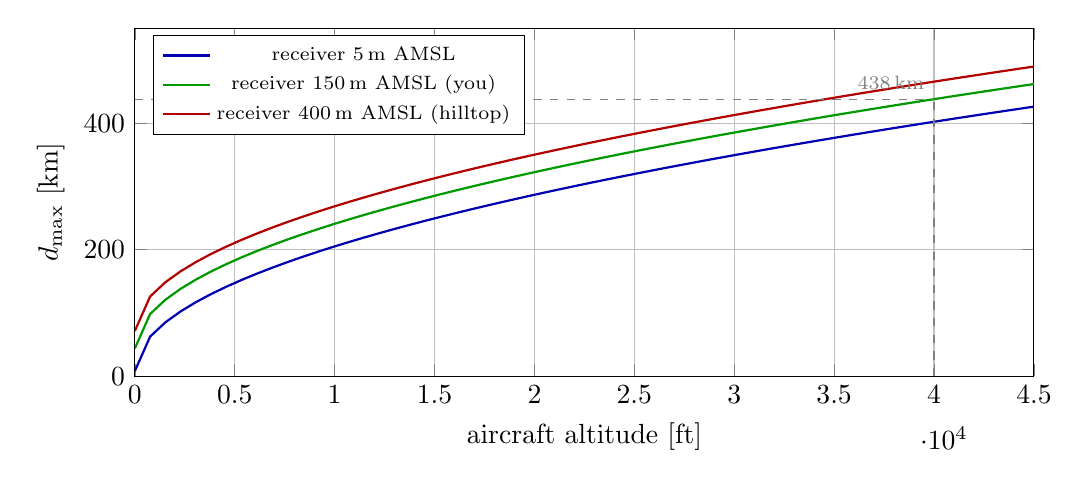
\begin{tikzpicture}
\begin{axis}[
    width=13cm, height=6cm,
    xlabel={aircraft altitude [\si{ft}]},
    ylabel={$d_{\max}$ [\si{km}]},
    xmin=0, xmax=45000,
    ymin=0, ymax=550,
    grid=both, minor grid style={line width=.1pt,draw=gray!20},
    legend style={at={(0.02,0.98)}, anchor=north west, font=\scriptsize},
    xtick distance=5000,
]
% Receiver at 5 m
\addplot[thick, blue!70!black, domain=0:45000, samples=60]
  {sqrt(2*6371*5/1000) + sqrt(2*6371*(x*0.3048)/1000)};
\addlegendentry{receiver \SI{5}{m} AMSL}
% Receiver at 150 m
\addplot[thick, green!60!black, domain=0:45000, samples=60]
  {sqrt(2*6371*150/1000) + sqrt(2*6371*(x*0.3048)/1000)};
\addlegendentry{receiver \SI{150}{m} AMSL (you)}
% Receiver at 400 m
\addplot[thick, red!70!black, domain=0:45000, samples=60]
  {sqrt(2*6371*400/1000) + sqrt(2*6371*(x*0.3048)/1000)};
\addlegendentry{receiver \SI{400}{m} AMSL (hilltop)}
% Marker at your typical operating point
\draw[dashed, gray] (axis cs:40000,0) -- (axis cs:40000,438);
\draw[dashed, gray] (axis cs:0,438) -- (axis cs:40000,438);
\node[font=\scriptsize, gray, anchor=south east] at (axis cs:40000,438) {\SI{438}{km}};
\end{axis}
\end{tikzpicture}
\end{center}

%═══════════════════════════════════════════════════════════════════
\section{Atmospheric refraction --- the $\tfrac{4}{3}$ earth}\label{sec:refraction}
%═══════════════════════════════════════════════════════════════════

Real air bends radio waves gently downward because its refractive index
falls with altitude.  The standard engineering shortcut is to pretend
the earth has a larger effective radius $\tilde R = k R$, with $k = 4/3$
under standard atmospheric conditions (Bean \& Dutton, 1966).  Plug
$\tilde R = \SI{8493}{km}$ into \eqref{eq:horizon} and every range grows by
$\sqrt{4/3} \approx 1.155$:
\[
d_{\max}^{\text{refr}} \;\approx\; \SI{506}{km}\quad\text{for our \SI{150}{m}\,+\,\SI{40000}{ft} case}.
\]
Under a strong tropospheric temperature inversion the effective $k$ can
climb toward $\infty$ (a duct); under sub-refractive conditions it can
drop below 1.  Both are covered in \S\ref{sec:sideeffects}.

%═══════════════════════════════════════════════════════════════════
\section{Free-space link budget}\label{sec:link}
%═══════════════════════════════════════════════════════════════════

Geometry tells us whether the signal \emph{can} arrive.  The link budget
tells us whether it can also be \emph{decoded}.  Free-space path loss
grows with the square of distance:
\begin{equation}
L_{\text{FSPL}} \;=\; \biggl(\frac{4 \pi d f}{c}\biggr)^{\!2}
\quad\Longleftrightarrow\quad
L_{\text{dB}} \;=\; 20 \log_{10}\!\biggl(\frac{4 \pi d f}{c}\biggr).
\end{equation}
At $f = \SI{1090}{MHz}$ ($\lambda = \SI{27.5}{cm}$) and $d = \SI{400}{km}$
this evaluates to \SI{145}{dB}.

A typical link budget for an airliner squitter reaching your setup:

\begin{center}
\begin{tabular}{l r}
\toprule
Term                                                   & Value            \\
\midrule
Transponder EIRP (Class A: 250 W)                      & \SI{54}{dBm}     \\
Aircraft antenna gain toward horizon (below-fuselage lobe) & $+\SI{3}{dBi}$   \\
Free-space loss at \SI{400}{km}                        & $-\SI{145}{dB}$  \\
Receiver antenna gain (quarter-wave whip / dipole)     & $+\SI{2}{dBi}$   \\
\midrule
Received signal at receiver input                      & $-\SI{86}{dBm}$  \\
Noise floor (\SI{2}{MHz} BW, SDR + LNA, NF \SI{1}{dB}) & $-\SI{111}{dBm}$ \\
\midrule
\textbf{Link margin}                                   & $+\SI{25}{dB}$   \\
\bottomrule
\end{tabular}
\end{center}

The decode threshold on consumer SDR + LNA sits around $-\SI{95}{dBm}$
(empirically; dump1090-fa's own decoder is even more sensitive for
strong preambles).  Solving for the distance at which received power
drops to that threshold:
\[
L_{\text{dB}} \;\le\; 54 + 3 + 2 - (-95) \;=\; \SI{154}{dB}
\quad\Longrightarrow\quad d \;\lesssim\; \SI{1250}{km}.
\]
That is \emph{far} beyond the \SI{450}{km} geometric horizon.
Practically: on any decent hobby setup the geometry is what binds you,
not the link budget.  On a bare RTL-SDR without an LNA the noise
figure jumps to \SI{7}{dB}, the decode threshold moves to about
$-\SI{89}{dBm}$, and the link-budget-limited range drops to
about \SI{620}{km} --- \emph{still} beyond geometric.  Only when
combined with cable losses, antenna losses, and gain over-compression
(see \texttt{pipeline.tex}) does the budget start to bite before
geometry does.

%═══════════════════════════════════════════════════════════════════
\section{Diffraction, ducting, and other side effects}\label{sec:sideeffects}
%═══════════════════════════════════════════════════════════════════

\subsection{Knife-edge diffraction}

A signal that grazes an obstacle (ridgeline, building) diffracts around
it.  In the classical single-knife-edge model (Bullington 1947) the
extra loss compared to free-space is $\sim\!\SI{6}{dB}$ per Fresnel-zone
obstruction depth of $\nu = 1$, rising to $\sim\!\SI{20}{dB}$ at $\nu = 3$.
In practice a hilltop between you and a distant aircraft costs
\SIrange{10}{20}{dB} of link margin --- rarely enough to eliminate a
signal that would otherwise be decodable from cruise altitude, but
usually enough to weaken the marginal ones.

\subsection{Tropospheric ducting}

Under strong low-level temperature inversions (typical: warm summer
evenings after a hot day) refractivity gradients steepen enough that
radio waves get trapped in a leaky ``surface duct'' between two
atmospheric layers.  The effective earth radius briefly goes very
large or even to infinity, and hobby ADS-B stations near coasts
routinely report signals from \SIrange{700}{1000}{km} during these
events.  It's the same phenomenon that causes summertime UHF-TV DX.
For your inland location it happens a few times a year rather than
weekly.

\subsection{Sub-refraction and blocking}

The opposite --- steeply humid air ABOVE a dry layer --- pushes $k$
below~1 and the horizon gets closer than the geometric baseline.  This
is rare but real and typically knocks \SIrange{10}{20}{km} off maximum
range for a few hours.

\subsection{Multipath from the ground}

At \SI{1090}{MHz} the sea and flat terrain form specular reflectors.  The
sum of direct + reflected signal at your antenna oscillates with height
and range in a fringe pattern.  For a horizontally-polarized receiver
antenna this can add or subtract up to \SI{6}{dB} depending on where a
plane sits in the pattern.  It doesn't set the range limit --- it just
makes reception fluttery as the plane crosses the fringes.

\subsection{Ionospheric propagation? No}

The critical frequency of the F2 layer is typically
\SIrange{10}{15}{MHz}; 1090\,MHz sails straight through with negligible
bending.  ADS-B is a strictly line-of-sight-or-nothing band --- you
never get the intercontinental range you would at HF.  Sporadic-E also
cuts off well below 200\,MHz, so it doesn't help either.

\subsection{Doppler shift and relativity}

A jet at Mach 0.85 does about $v = \SI{260}{m/s}$ relative to a ground
receiver.  Doppler shift at 1090\,MHz:
\[
\Delta f \;=\; \frac{v}{c}\, f \;\approx\; \SI{945}{Hz}
              \;\approx\; \SI{0.9}{ppm}.
\]
That is a rounding error compared to typical SDR local-oscillator
drift of \SIrange{10}{50}{ppm}.  ADS-B is a burst-modulated signal
with wide preamble tolerance, so Doppler does not degrade decode
probability at all.

\medskip
Special-relativistic time dilation on board the aircraft:
\[
\frac{\Delta t}{t} \;=\; \frac{1}{2}\biggl(\frac{v}{c}\biggr)^{\!2}
\;\approx\; \num{4e-13}.
\]
Over the \SI{112}{\micro s} it takes to transmit a long squitter the
clock offset is $\sim\!\SI{4.5e-17}{s}$ --- irrelevant.

General-relativistic effect from sitting at \SI{12}{km} higher in
Earth's gravitational potential ($g h$):
\[
\frac{\Delta t}{t} \;=\; \frac{g h}{c^{2}}
\;\approx\; \num{1.3e-15}\quad\text{(clock runs faster by this fraction)}.
\]
Also irrelevant.  ADS-B works because burst timing tolerances are
enormous compared to any relativistic term.  Where relativity does
matter is on the transmitting satellite in GPS \emph{onboard} the
aircraft --- that's where the corrections have to be applied.  Not
here.

\subsection{Aircraft antenna pattern}

The transponder antenna is a quarter-wave monopole mounted underneath
the fuselage.  Its azimuthal pattern is roughly omni; the elevation
pattern has a broad lobe pointed at the ground plane of the aircraft,
a null pointing straight down, and secondary lobes at
\ang{5} to \ang{20} below the aircraft --- which happens to be exactly
the angle to a distant ground receiver at horizon range.  So aircraft
antenna gain \emph{helps} rather than hurts at long ranges, on the
order of \SIrange{2}{4}{dB} of extra received power vs the naive
isotropic assumption.

\subsection{Terrain, buildings, and vegetation}

Trier sits in the Moselle valley at \SIrange{125}{150}{m}, with hills
rising steeply to \SI{400}{m} on both sides (Petrisberg to the east,
Markusberg to the south, Grüneberg to the northwest).  A receiver on
one of these hilltops adds another \SIrange{25}{30}{km} of horizon
distance --- more useful than any indoor upgrade you can do.  The
Sûre valley opening toward Luxembourg to the west gives you a
comparatively distant western horizon.

Buildings, trees, and other antennas cause hard shadowing at
1090\,MHz.  Concrete walls attenuate \SIrange{20}{30}{dB}; wet
deciduous canopies \SIrange{10}{12}{dB} per meter of foliage
penetration.  A rooftop mount clear of surrounding structures
routinely doubles decoded-frame counts vs an indoor antenna at the
same nominal height.

%═══════════════════════════════════════════════════════════════════
\section{Summary}\label{sec:summary}
%═══════════════════════════════════════════════════════════════════

\begin{center}
\begin{tabular}{l r}
\toprule
Physical limit                                                        & Range              \\
\midrule
Geometric horizon, \SI{150}{m} rx, \SI{40000}{ft} tx                  & \SI{438}{km}       \\
+ standard $\tfrac{4}{3}$ earth (atmospheric refraction)              & \SI{506}{km}       \\
Rural hilltop rx at \SI{400}{m}, same aircraft                         & \SI{489}{km} geo   \\
Same, with refraction                                                 & \SI{565}{km}       \\
Consumer SDR + LNA link-budget cap alone                              & $\sim\!\SI{1250}{km}$ \\
Bare RTL-SDR (no LNA) link-budget cap alone                           & $\sim\!\SI{620}{km}$  \\
Occasional tropospheric ducting event                                  & \SIrange{700}{1000}{km} \\
\bottomrule
\end{tabular}
\end{center}

\paragraph{Take-away.}
From your rooftop, expect a hard ceiling near \SI{500}{km} on typical
days.  On a hilltop hike with the antenna up high, \SI{550}{km} is
reachable when a plane happens to be at 45\,000 ft.  Signals beyond
\SI{600}{km} are always either a ducting event (check the local
tropospheric propagation forecast) or a receiver location much higher
than \SI{150}{m} AMSL.  The plugin's Farthest indicator (top-left HUD)
is the number to watch --- when it exceeds \SI{500}{km} on an ordinary
day, that alone is the tell that unusual propagation is happening.

\end{document}
